\subsection{Emergency Mixed Head on with Converging}\label{s:testEmergencyMixed}

    \noindent\paragraph{Scenario:} \emph{Four UAS} are flying in an \emph{uncontrolled airspace} (altitude $\le$ 500 ft. Above the Ground Level) missions defined in (tab. \ref{tab:missionSetupEmergencyMixedScenario}). All UAS are in the \emph{Navigation mode} with active \emph{ADS-B In}, receiving \emph{position notifications} from each other. Cruising altitude is sufficient for \emph{horizontal separation} (50-100 ft. Above the Ground Level).
    
    
    \begin{table}[H]
        \centering
        \begin{tabular}{c||c|c||c}
            \multirow{2}{*}{UAS} &\multicolumn{2}{c||}{Position} & \multirow{2}{*}{$\mathscr{WP}_1$} \\\cline{2-3}
              & $[x,y,z]$           & $[\theta,\varpi,\psi]$           & \\\hline\hline
            1 & $[0,20,0]^T $       & $[0^\circ,0^\circ,0^\circ]^T$    & $[45,20,0]^T$\\\hline 
            2 & $[40,20,0]^T $       & $[0^\circ,0^\circ,180^\circ]^T$    & $[-5,20,0]^T$\\\hline 
            3 & $[20,0,0]^T $       & $[0^\circ,0^\circ,90^\circ]^T$    & $[20,45,0]^T$\\\hline 
            4 & $[20,40,0]^T $       & $[0^\circ,0^\circ,-90^\circ]^T$  & $[45,20,0]^T$\\ 
        \end{tabular}
        \caption{Mission setup for \emph{Emergency mixed} scenario.}
        \label{tab:missionSetupEmergencyMixedScenario}
    \end{table}
    
    \begin{note}
        \emph{Collision point} is expected at $\mathscr{C}=[20,20,0]^T$
    \end{note}
    
    \noindent \paragraph{Main Goal:} Show \emph{multiple non-cooperative intruders avoidance capability} in \emph{uncontrolled} airspace.
    
    \noindent \paragraph{Acceptance criteria:}
    \begin{enumerate}
        \item \emph{Proper avoidance mode invocation} - when an  \emph{intruder intersection model} impact the \emph{Avoidance Grid}, UAS system will switch to an \emph{Emergency avoidance mode}.
        
        \item\emph{Minimal safety margin distance} $\ge$ $0 m$.
        
        \item Each \emph{UAS} will reach own goal waypoint (tab. \ref{tab:missionSetupEmergencyMixedScenario}).
    \end{enumerate}
    
    
    \noindent\paragraph{Testing setup:} The \emph{standard test setup} for each UAS defined in (tab \ref{tab:testMovementOrientations}, \ref{tab:testUASBasicParameters}, \ref{tab:testNavigationGridBasic}, \ref{tab:testAvoidanceGridBasic}, \ref{tab:testUASColoring}) is used with following without parameter override.

    \emph{Intruder intersection} model has been chosen depending on UAS (tab. \ref{tab:aboidanceParametersForEmergencyMixedScenario}). Each UAS is equipped with \emph{ADS-B In/Out} sensor obtaining/distributing following information:
    \begin{enumerate}
        \item \emph{Position} - in operational section coordinate frame.
        \item \emph{Velocity} - vector representation in given coordinate frame.
        \item \emph{Class size} - class body radius based on UAS propulsion and size.
        \item \emph{Safety margin set} - set of safety margins for different collision cases.
    \end{enumerate}
    
    \emph{Avoidance parameters} for \emph{Emergency mixed scenario} are given in (tab. \ref{tab:aboidanceParametersForEmergencyMixedScenario}). Each UAS has different \emph{intruder model} and separation combination. Each UAS has same speed set to $1 m s^{-1}$. None of UAS has the \emph{Right of The Way}. 
    
    \emph{Safety margin} is considered as sum of both participants \emph{near miss margins}. In this case default safety margin is considered as $1.2$  $m$.
    
    \begin{table}[H]
        \centering
        \begin{tabular}{c||c|c|c||c|c||c}
            \multirow{2}{*}{UAS} & \multicolumn{3}{c||}{Parameters} & \multicolumn{2}{c||}{Margins} & \multirow{2}{*}{Separation}\\\cline{2-6}
                                 & velocity & intruder model & ROW        & body & safety                                        \\\hline\hline
            1                    & 1        & body + spread  & false            & 0.3         & 0.6           & horizontal       \\\hline
            2                    & 1        & body (timed)   & false            & 0.3         & 0.6           & vertical         \\\hline
            3                    & 1        & body (timed)   & false            & 0.3         & 0.6           & horizontal       \\\hline
            2                    & 1        & body + spread  & false            & 0.3         & 0.6           & vertical         \\
        \end{tabular}
        \caption{Avoidance parameters for  \emph{Emergency mixed} scenario.}
        \label{tab:aboidanceParametersForEmergencyMixedScenario}
    \end{table}
    
    \begin{note}
        Each \emph{UAS} use different intruder intersection models and primary \emph{separations} (defined in tab. \ref{tab:aboidanceParametersForEmergencyMixedScenario}).  UAS reactions are based on primary \emph{Separation} mode, intruders intersection models this is reflected on major axial deviations in (fig. \ref{fig:testCaseEmergencyMixedTrajectoryTracking}) and summarized in \emph{path tracking} deviation (tab. \ref{tab:pathTrackingParametersForEmergencyMixed}).
    \end{note}
    
    \noindent\paragraph{Simulation Run:} Notable moments from the simulation run (fig. \ref{fig:testCaseEmergencyMixed}) are following:
    
    \begin{enumerate}
        \item \emph{Situation detection} (fig. \ref{fig:emergencyMultipleSituationDetection}) - UAS 1 (blue) is detecting UAS 2 (cyan), UAS 3 (green), and UAS 4 (black) as possible intruders. There are multiple converging and head on approaches depending on mutual positions (UAS and \emph{angle of approach}). There exist at least one \emph{converging case} where each UAS has \emph{Right of the way}. Each UAS creates intruder intersection models depending on the intruder configuration (tab. \ref{tab:aboidanceParametersForEmergencyMixedScenario}). Each UAS enters into the \emph{Emergency avoidance mode} independently, when at least one trajectory is constrained in the \emph{avoidance grid}. 
        
        \item \emph{Before near miss} (fig. \ref{fig:emergencyMultipleBeforeNearMiss}) - all \emph{UAS} are in \emph{emergency avoidance mode}, using various \emph{separation modes} and \emph{intruder intersection models}. Each UAS is performing its own avoidance maneuver, constantly checking other intruders. If same separation and same intruder model was used, there will be virtual roundabout.
            
        \item \emph{After near miss} (fig. \ref{fig:emergencyMultipleAfterNearMiss}) - all \emph{UAS} avoided each other which is covered in \emph{safety margin performance} (fig. \ref{fig:testCaseMultipleAvoidancePerformance}) and (tab. \ref{tab:testCaseEmergencyMixedSafetyMarginDistances}).
        
        \item \emph{Situation resolution} (fig. \ref{fig:emergencyMultipleSituationReslution}) - all \emph{UAS}
        returns to \emph{Navigation mode} correcting \emph{altitude} first and continuing to assigned waypoints.
    \end{enumerate}
    
    \begin{figure}[H]
        \centering
        \begin{subfigure}{0.48\textwidth}
        	\centering
            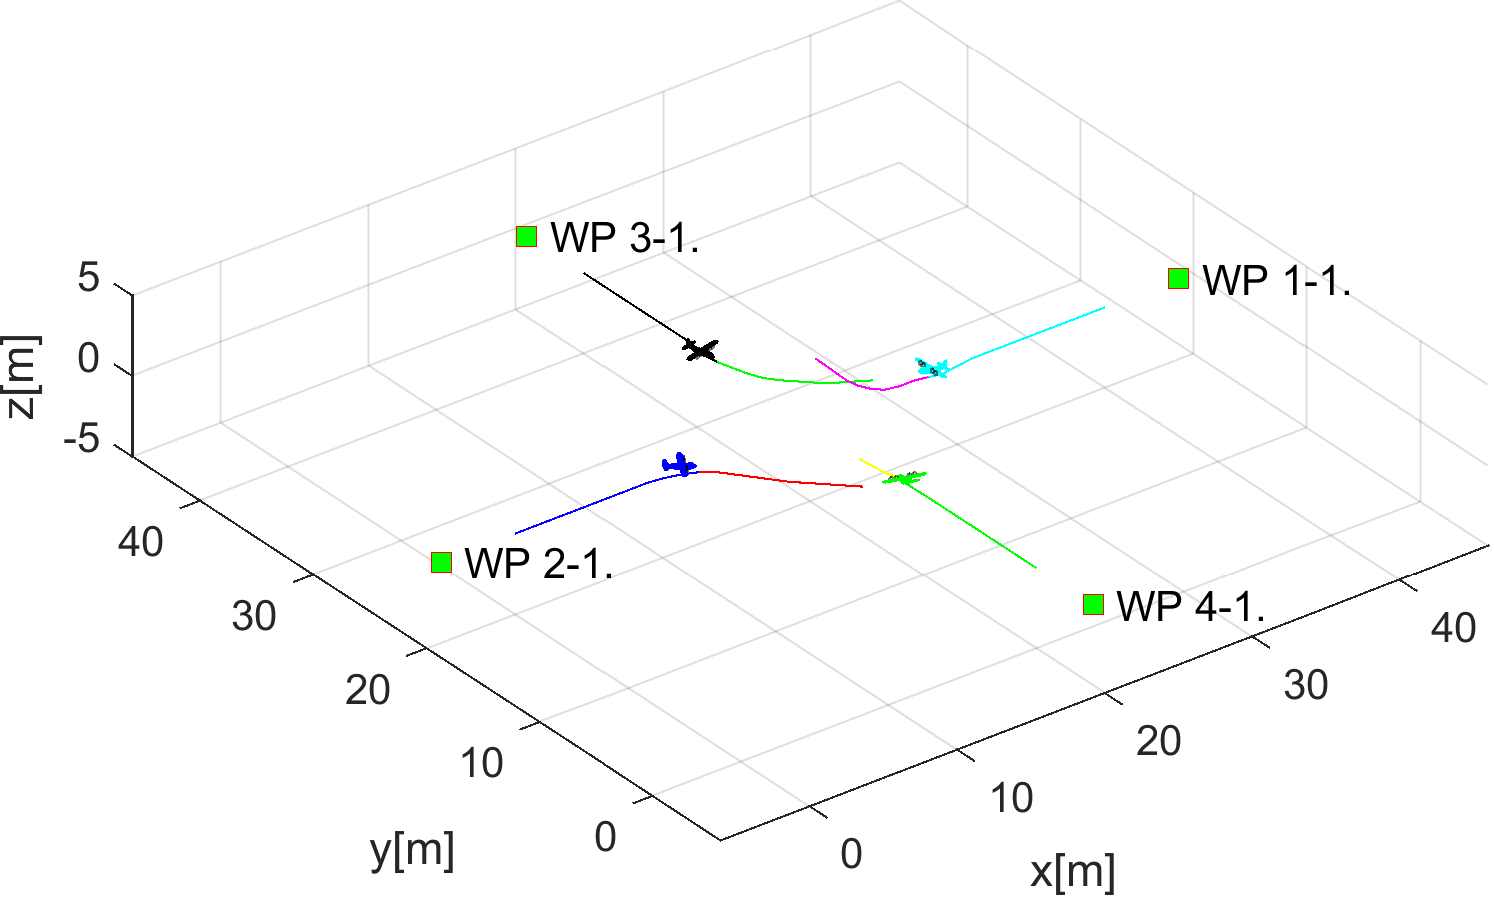
\includegraphics[width=0.9\linewidth]{\FIGDIR/NS039UtmEmergencyHeadOnMultiple00012}
            \caption{Situation detection.}
            \label{fig:emergencyMultipleSituationDetection}
        \end{subfigure}
        \begin{subfigure}{0.48\textwidth}
        	\centering
            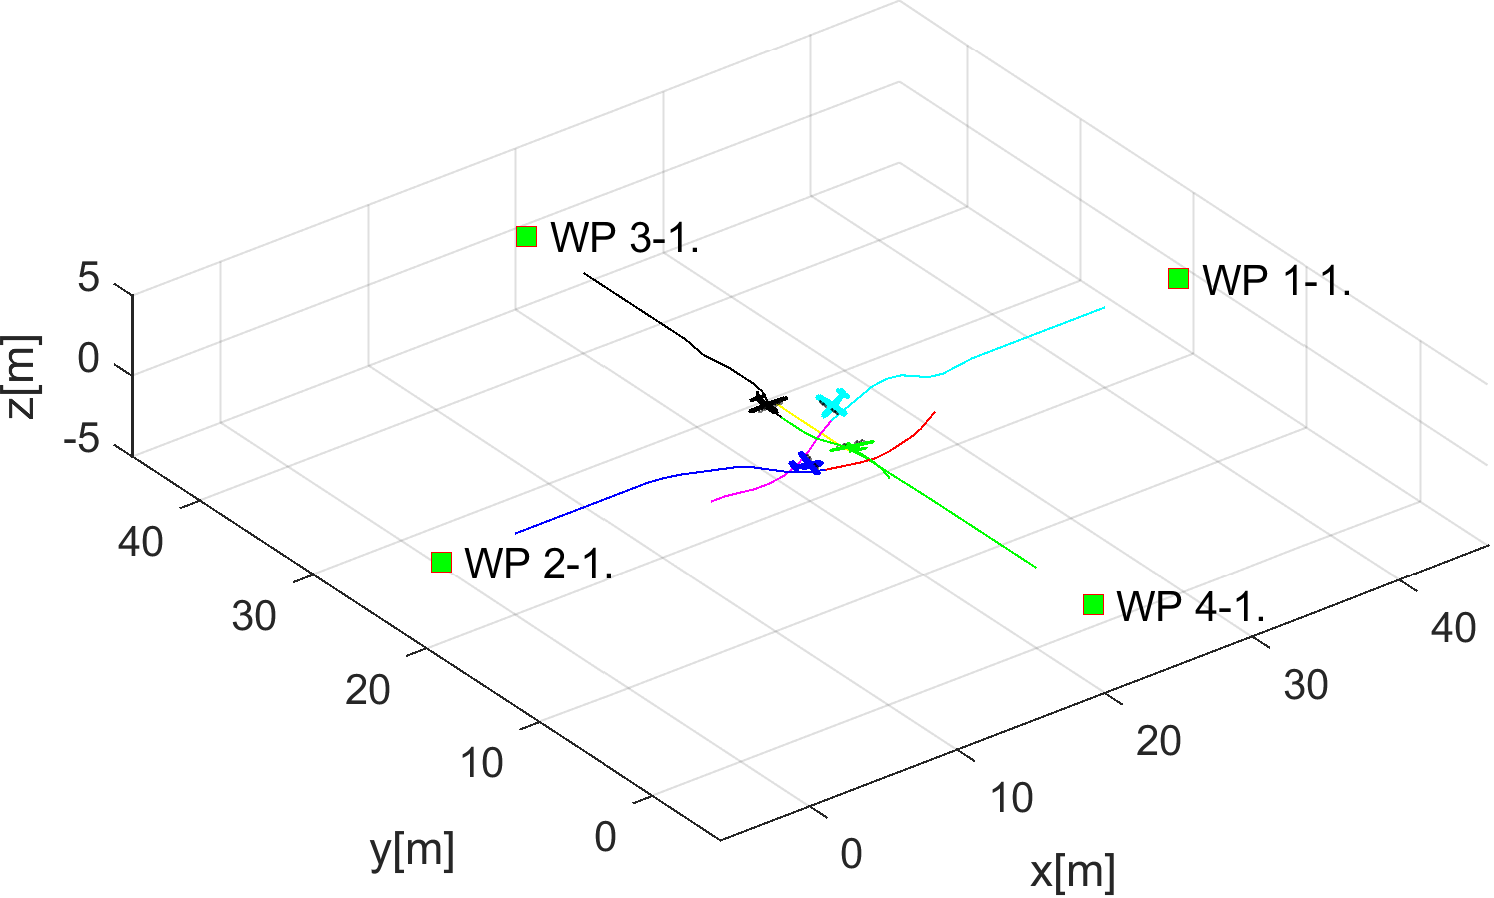
\includegraphics[width=0.9\linewidth]{\FIGDIR/NS040UtmEmergencyHeadOnMultiple00019} 
            \caption{Before near miss.}
            \label{fig:emergencyMultipleBeforeNearMiss}
        \end{subfigure}
        \\
        \begin{subfigure}{0.48\textwidth}
        	\centering
            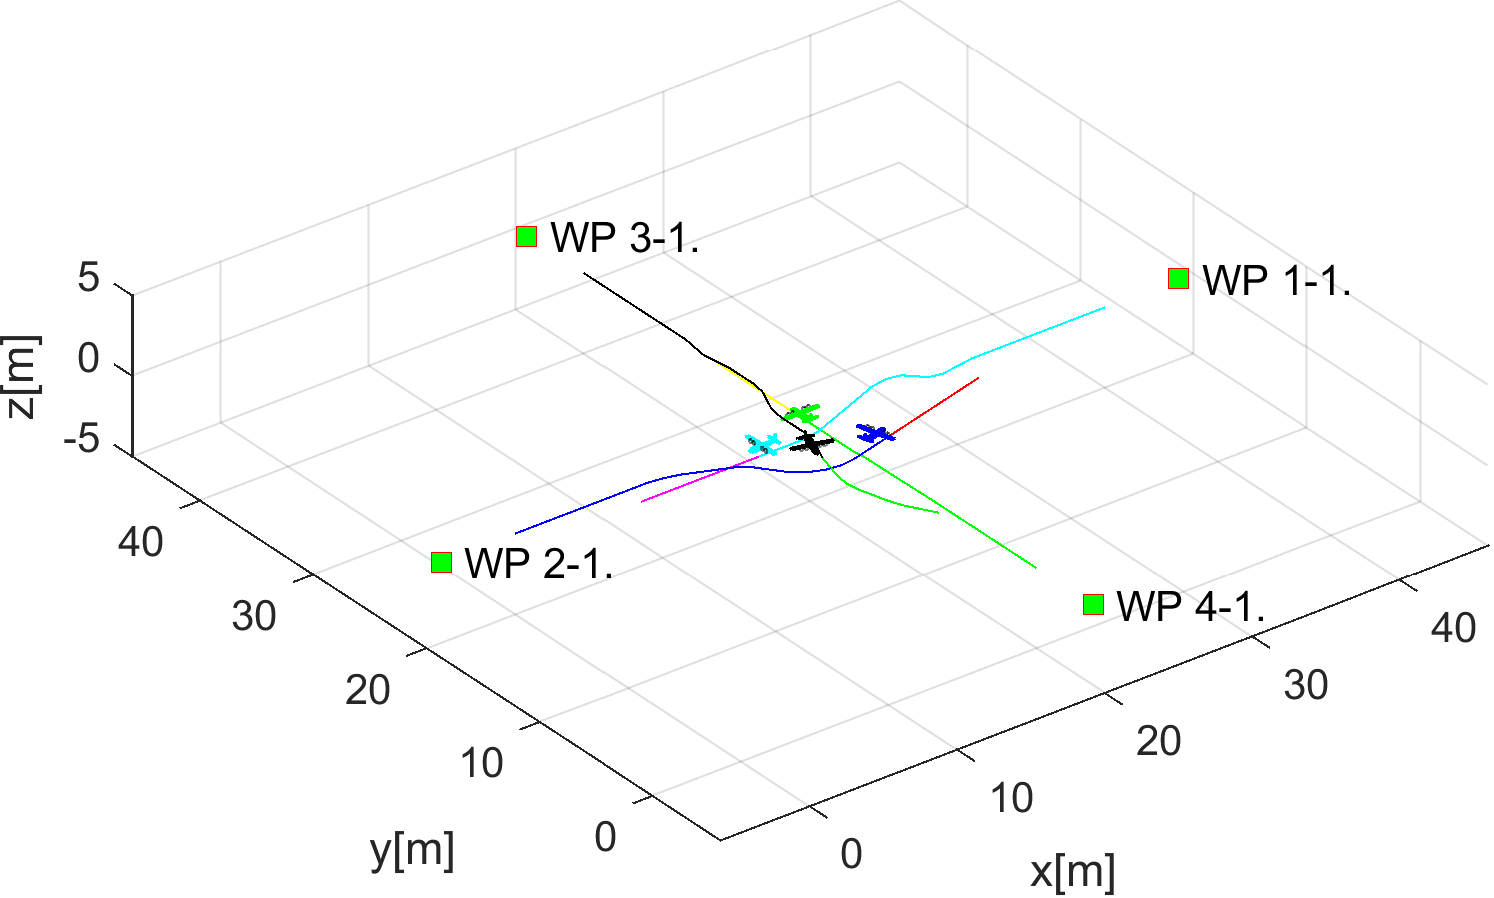
\includegraphics[width=0.9\linewidth]{\FIGDIR/NS041UtmEmergencyHeadOnMultiple00024} 
            \caption{After near miss.}
            \label{fig:emergencyMultipleAfterNearMiss}
        \end{subfigure}
        \begin{subfigure}{0.48\textwidth}
        	\centering
            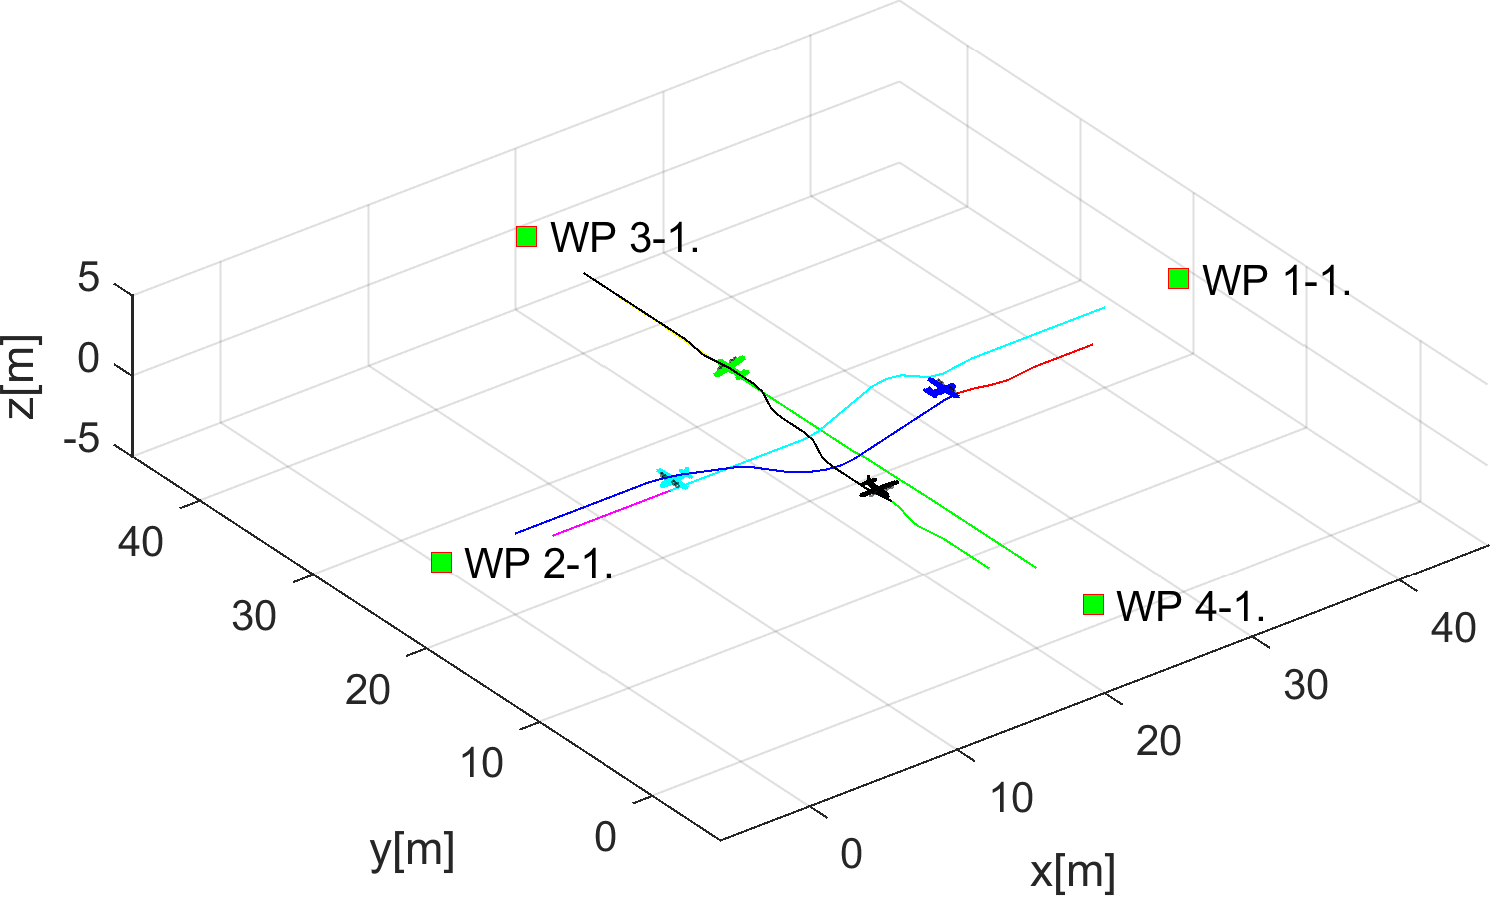
\includegraphics[width=0.9\linewidth]{\FIGDIR/NS042UtmEmergencyHeadOnMultiple00030} 
            \caption{Situation resolution.}
            \label{fig:emergencyMultipleSituationReslution}
        \end{subfigure}
        \caption{Test scenario for \emph{Emergency mixed} situation with \emph{self-separation mode}.}
        \label{fig:testCaseEmergencyMixed}
    \end{figure}
    
    \paragraph{Distance to Safety Margin Evolution:} There is need to compare mutual distance between each UAS. The graph (fig. \ref{fig:testCaseMultipleAvoidancePerformance}) shows six figures for each \emph{UAS systems} mutual distance (blue line) in this scenario. The \emph{Safety Margin} (red line) ($1.2$ $m$) was not breached for any pair (case). 
    
    The \emph{Proper avoidance invocation} is shown when UAS systems are getting closer to each other and then they start separation phase (Emergency avoidance mode).
            
    \begin{figure}[H]
        \centering
        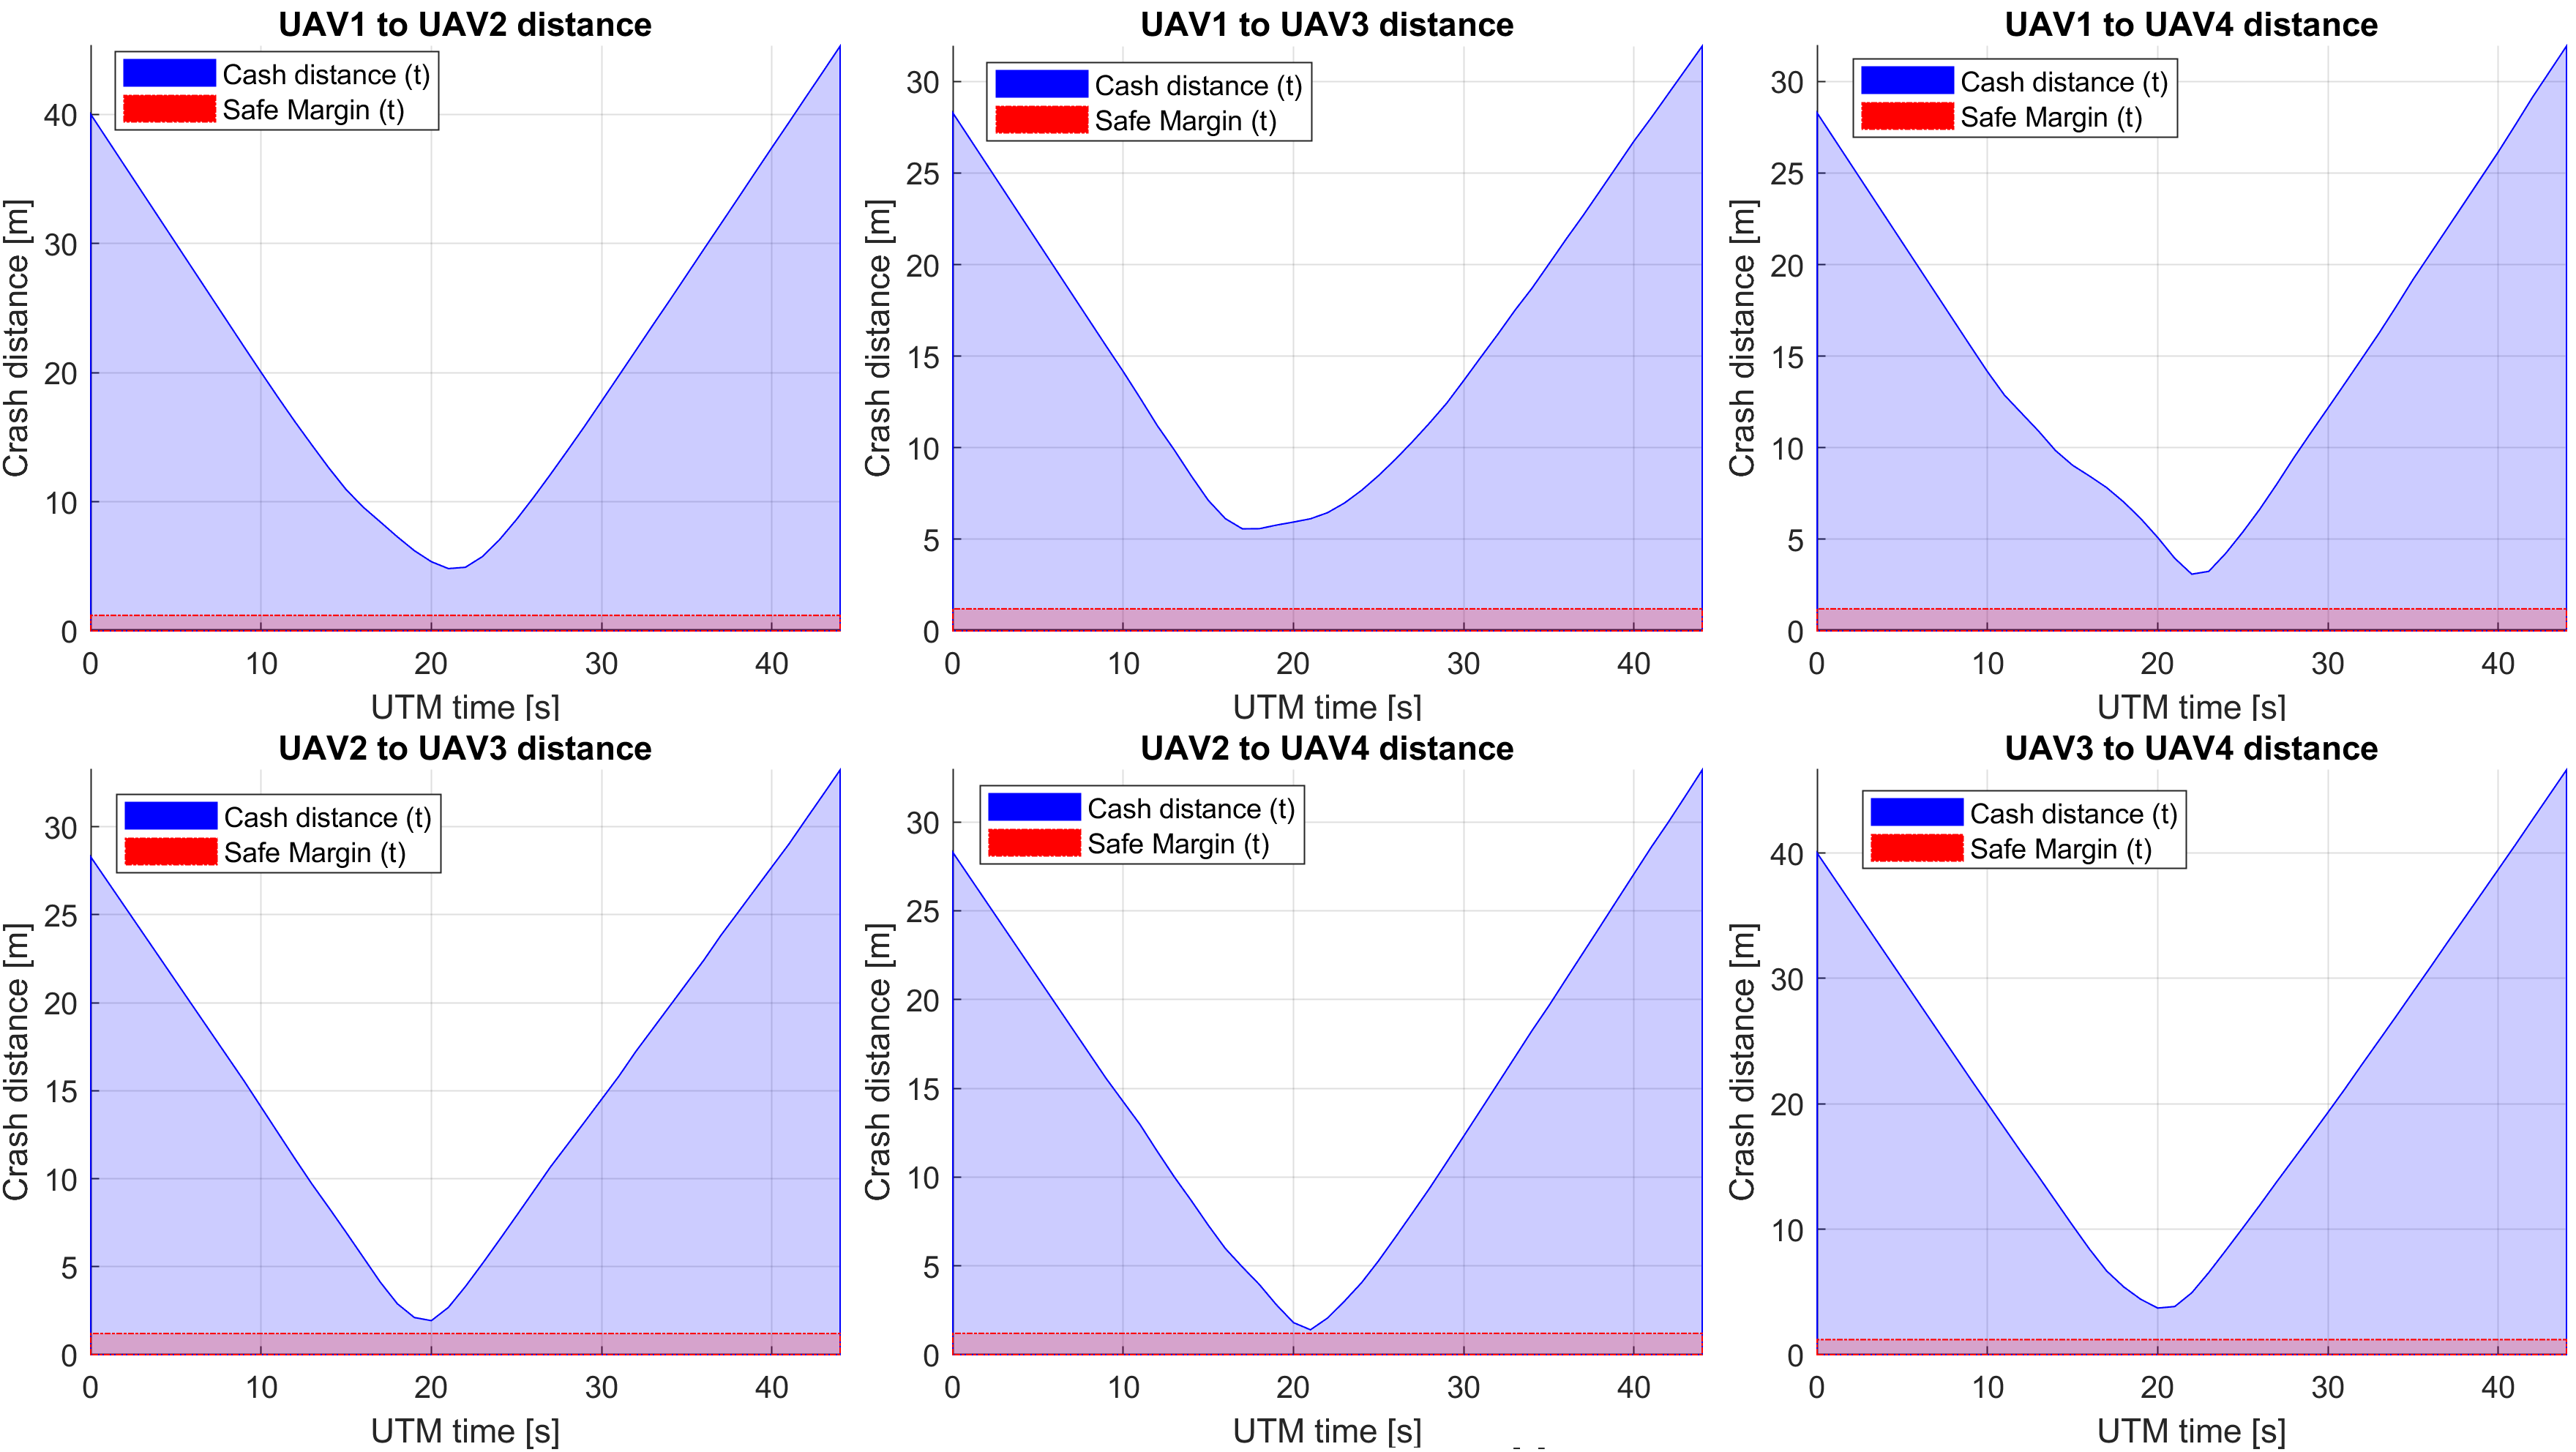
\includegraphics[width=0.9\linewidth]{\FIGDIR/NS043UtmEmergencyHeadOnMultiplePerformance} 
        \caption{Distance to safety margin evolution for \emph{emergency mixed scenario}.}
        \label{fig:testCaseMultipleAvoidancePerformance}
    \end{figure}
    
    \paragraph{Distance to Safety Margin Peaks:} Minimal and Maximal mutual distance to safety margin is summarized in (tab. \ref{tab:testCaseEmergencyMixedSafetyMarginDistances}). There is no detected breach for any combination. 
    
    The \emph{closest to collision} is UAS pair $2-4$ with mutual safety margin only $0.2019$ $m$. On the other side is UAS pair $1-3$ with mutual safety margin $4.3721$ $m$. 
    
    The \emph{minimal distance to safety margin}  $\ge$ 0 which means that the \emph{safety condition} is fulfilled. 
    
    \begin{table}[H]
        \centering
        \begin{tabular}{c||c|c|c}
            \multirow{2}{*}{UAS:} & \multicolumn{3}{c}{Distance to Safety Margin} \\ \cline{2-4} 
                      & min          & max         & breach         \\ \hline\hline
                1-2   & 3.6231       & 44.0831     & false          \\ \hline
                1-3   & 4.3721       & 30.7300     & false          \\ \hline
                1-4   & 1.8959       & 30.7331     & false          \\ \hline
                2-3   & 0.7331       & 32.0266     & false          \\ \hline
                2-4   & 0.2019       & 31.7282     & false          \\ \hline
                3-4   & 2.5171       & 45.4257     & false          \\ 
        \end{tabular}
        \caption{Distance to safety margin peaks for \emph{emergency mixed scenario}.}
        \label{tab:testCaseEmergencyMixedSafetyMarginDistances}
    \end{table}
    
    \noindent\paragraph{Path Tracking Performance:} All waypoints (Green numbered squares) for all UAS have been reached (fig. \ref{fig:testCaseEmergencyMixedTrajectoryTracking}). \emph{Reference trajectories} (green dashed line) have been tracked by \emph{UAS real path} (blue solid line) almost all time. 
    
    Following observations can be made from \emph{path tracking} (fig. \ref{fig:testCaseEmergencyMixedTrajectoryTracking}) and \emph{preferred separations} (tab. \ref{tab:aboidanceParametersForEmergencyMixedScenario}):
    
    \begin{enumerate}
        \item UAS 1 (fig. \ref{fig:emergencyMixedPathTrackingUAS1}) is using \emph{horizontal separation} (y axis right) having \emph{preferred horizontal separation}.
        
        \item UAS 2 (fig. \ref{fig:emergencyMixedPathTrackingUAS2}) is using vertical separation (z axis up-down), having preferred vertical separation.
        
        \item UAS 3 (fig. \ref{fig:emergencyMixedPathTrackingUAS3}) is using horizontal/vertical separation (x right, z down), having preferred horizontal separation.  This UAS has used other than preferred separation type.
        
        \item UAS 4 (fig. \ref{fig:emergencyMixedPathTrackingUAS4}) is using horizontal separation (x-axis right/left), having preferred vertical separation. This UAS has used opposite separation type, than preferred.
    \end{enumerate}
    
    
    \begin{figure}[H]
        \centering
        \begin{subfigure}{0.48\textwidth}
        	\centering
            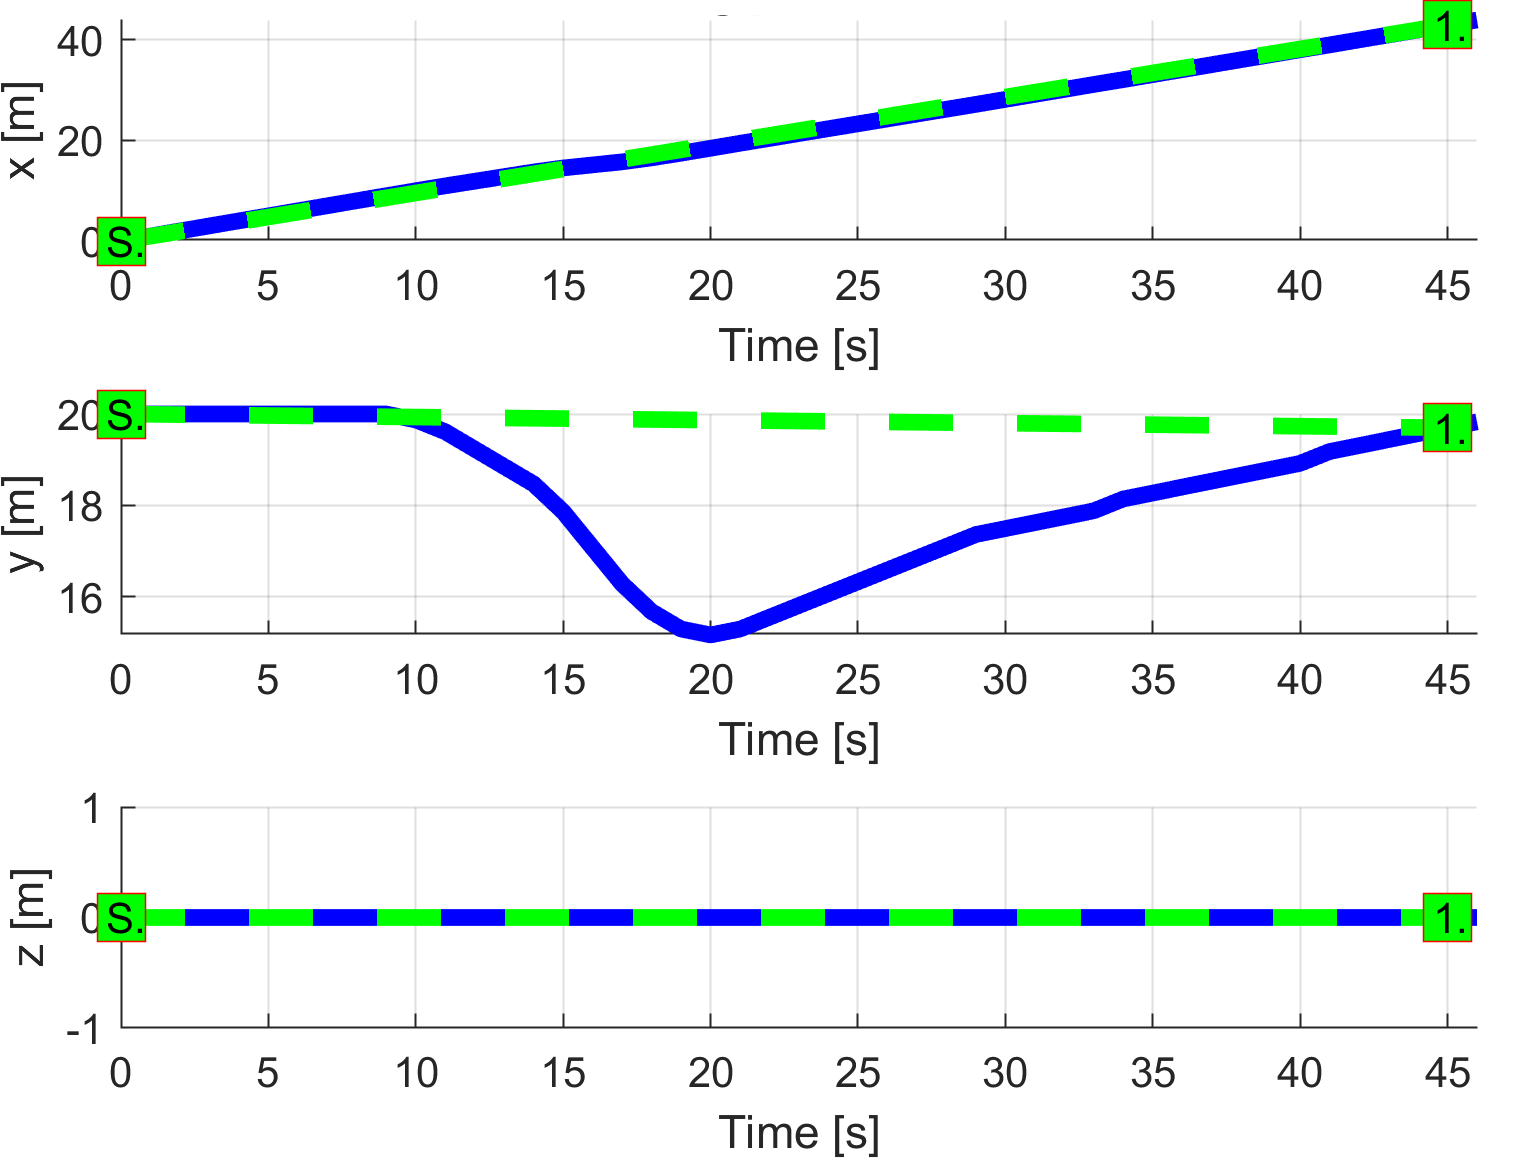
\includegraphics[width=0.9\linewidth]{\FIGDIR/NS044UtmEmergencyHeadOnMultipleUAV1PathFollowing}
            \caption{UAS 1.}
            \label{fig:emergencyMixedPathTrackingUAS1}
        \end{subfigure}
        \begin{subfigure}{0.48\textwidth}
        	\centering
            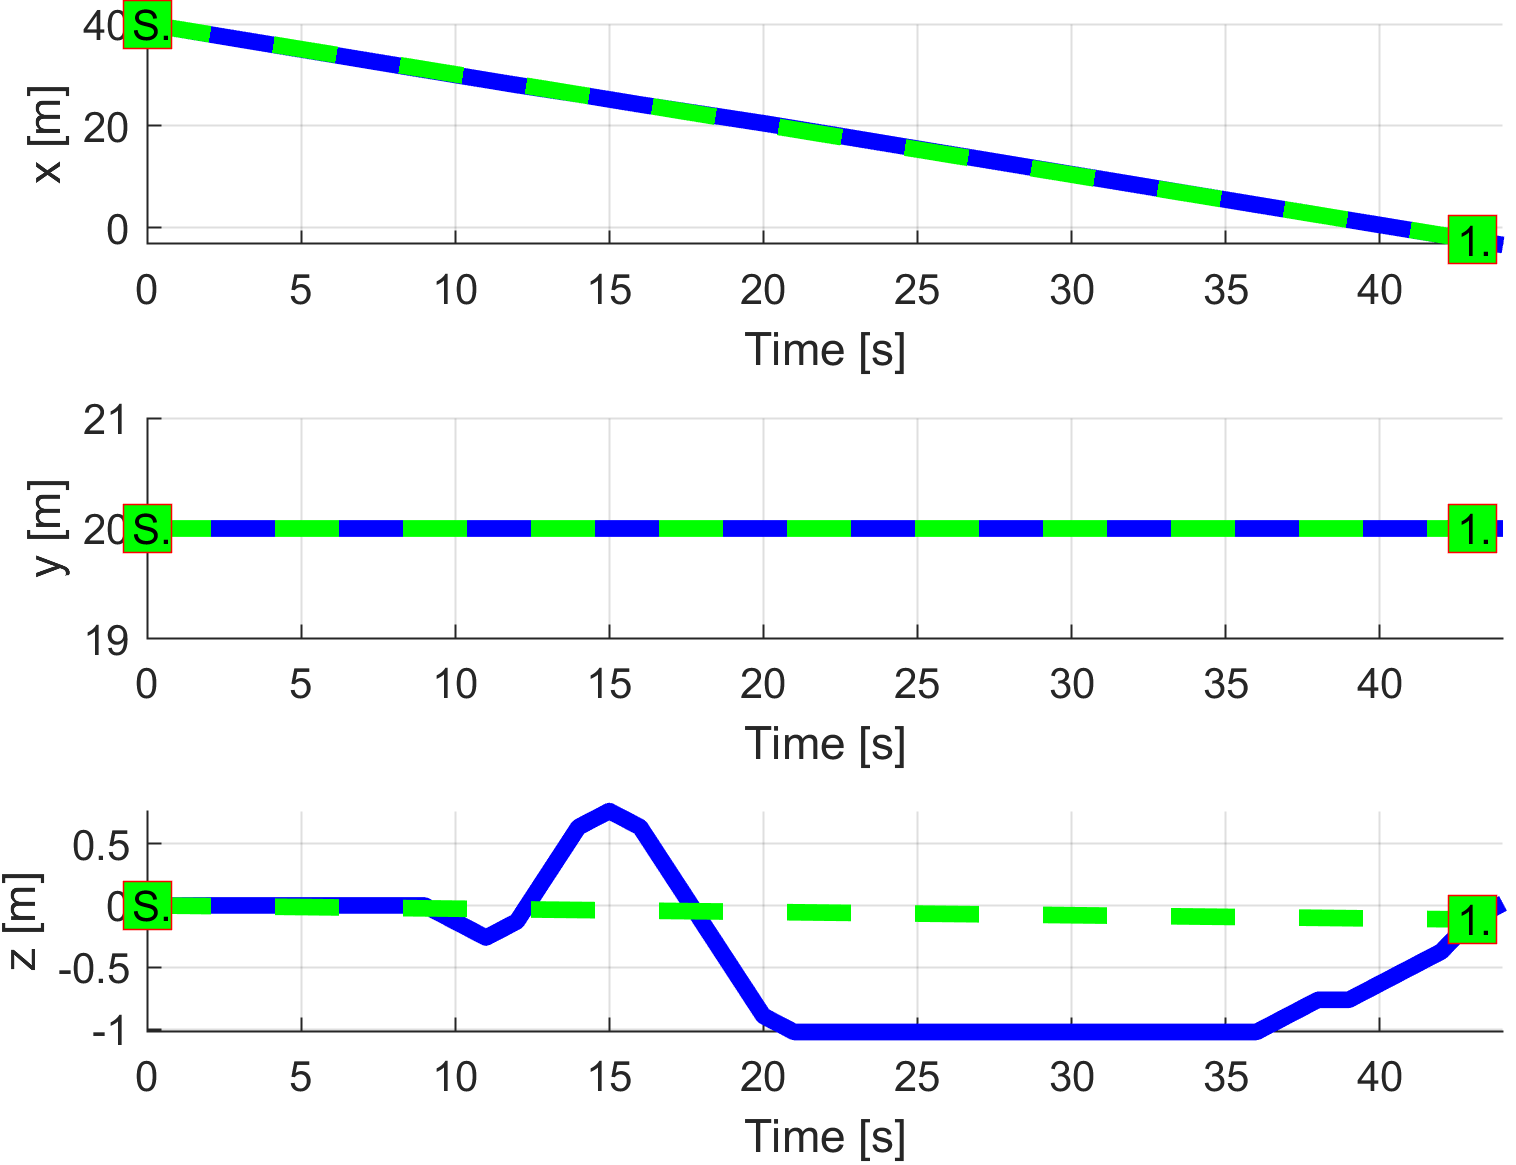
\includegraphics[width=0.9\linewidth]{\FIGDIR/NS045UtmEmergencyHeadOnMultipleUAV2PathFollowing} 
            \caption{UAS 2.}
            \label{fig:emergencyMixedPathTrackingUAS2}
        \end{subfigure}
        \\
        \begin{subfigure}{0.48\textwidth}
        	\centering
            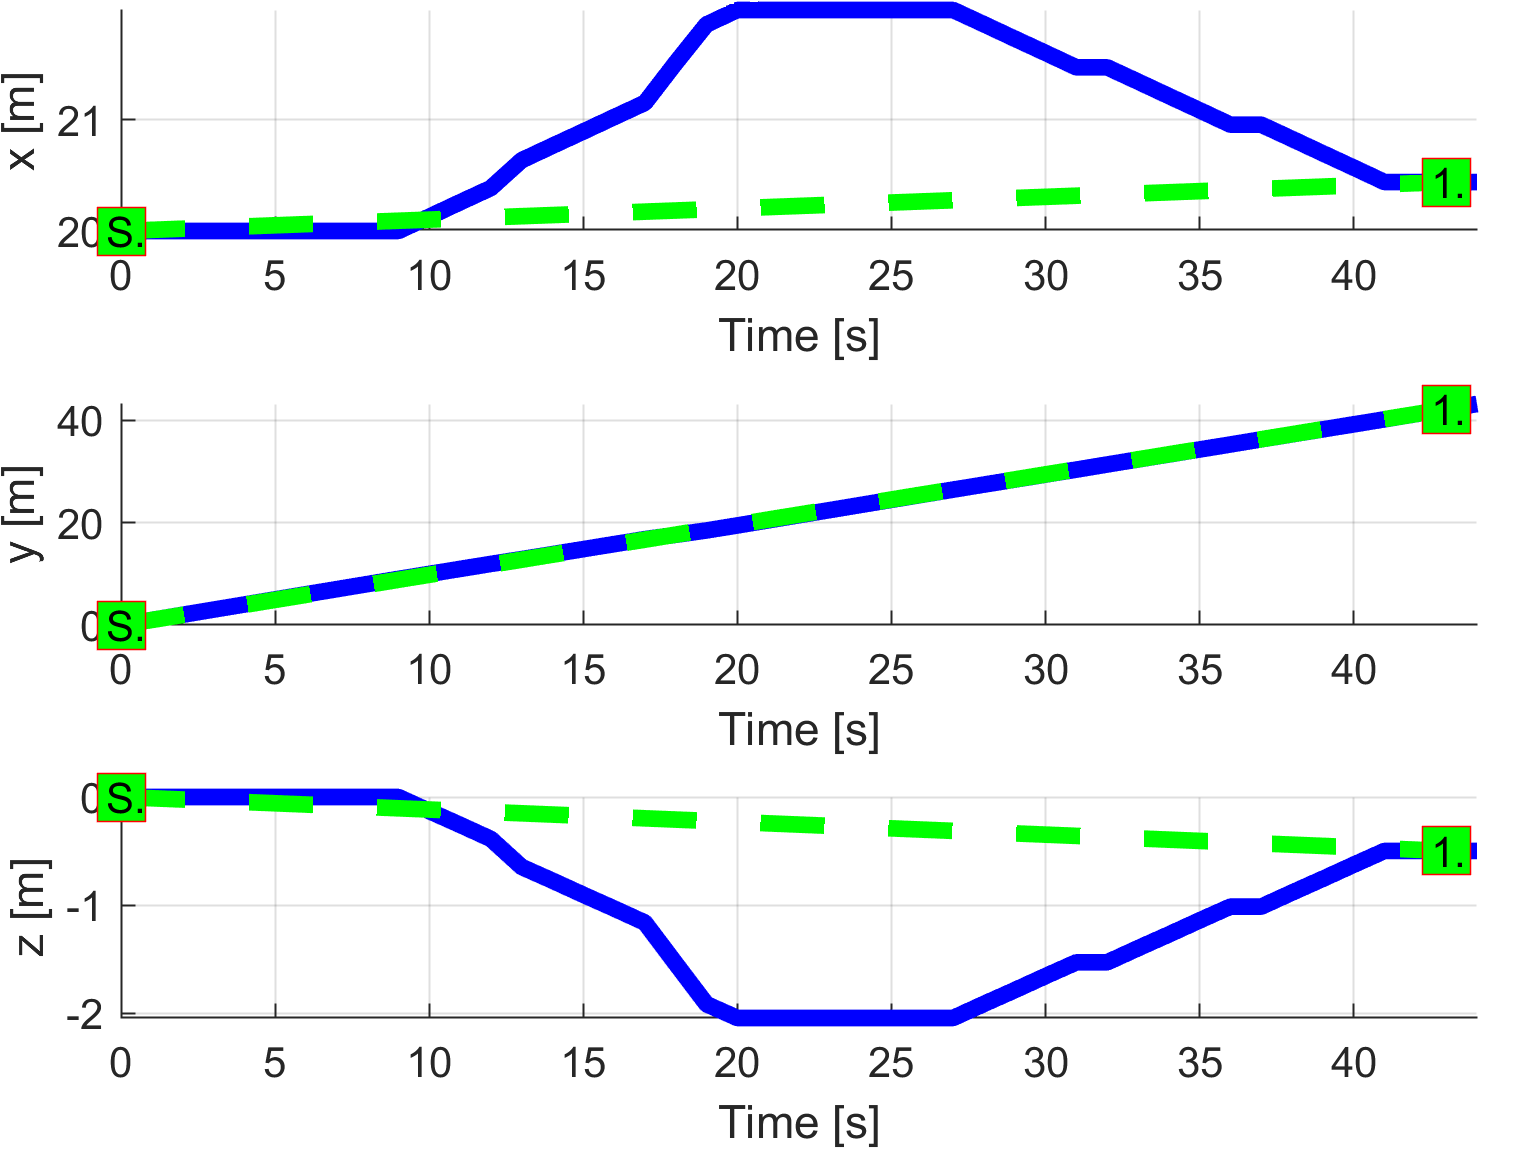
\includegraphics[width=0.9\linewidth]{\FIGDIR/NS046UtmEmergencyHeadOnMultipleUAV3PathFollowing} 
            \caption{UAS 3.}
            \label{fig:emergencyMixedPathTrackingUAS4}
        \end{subfigure}
        \begin{subfigure}{0.48\textwidth}
        	\centering
            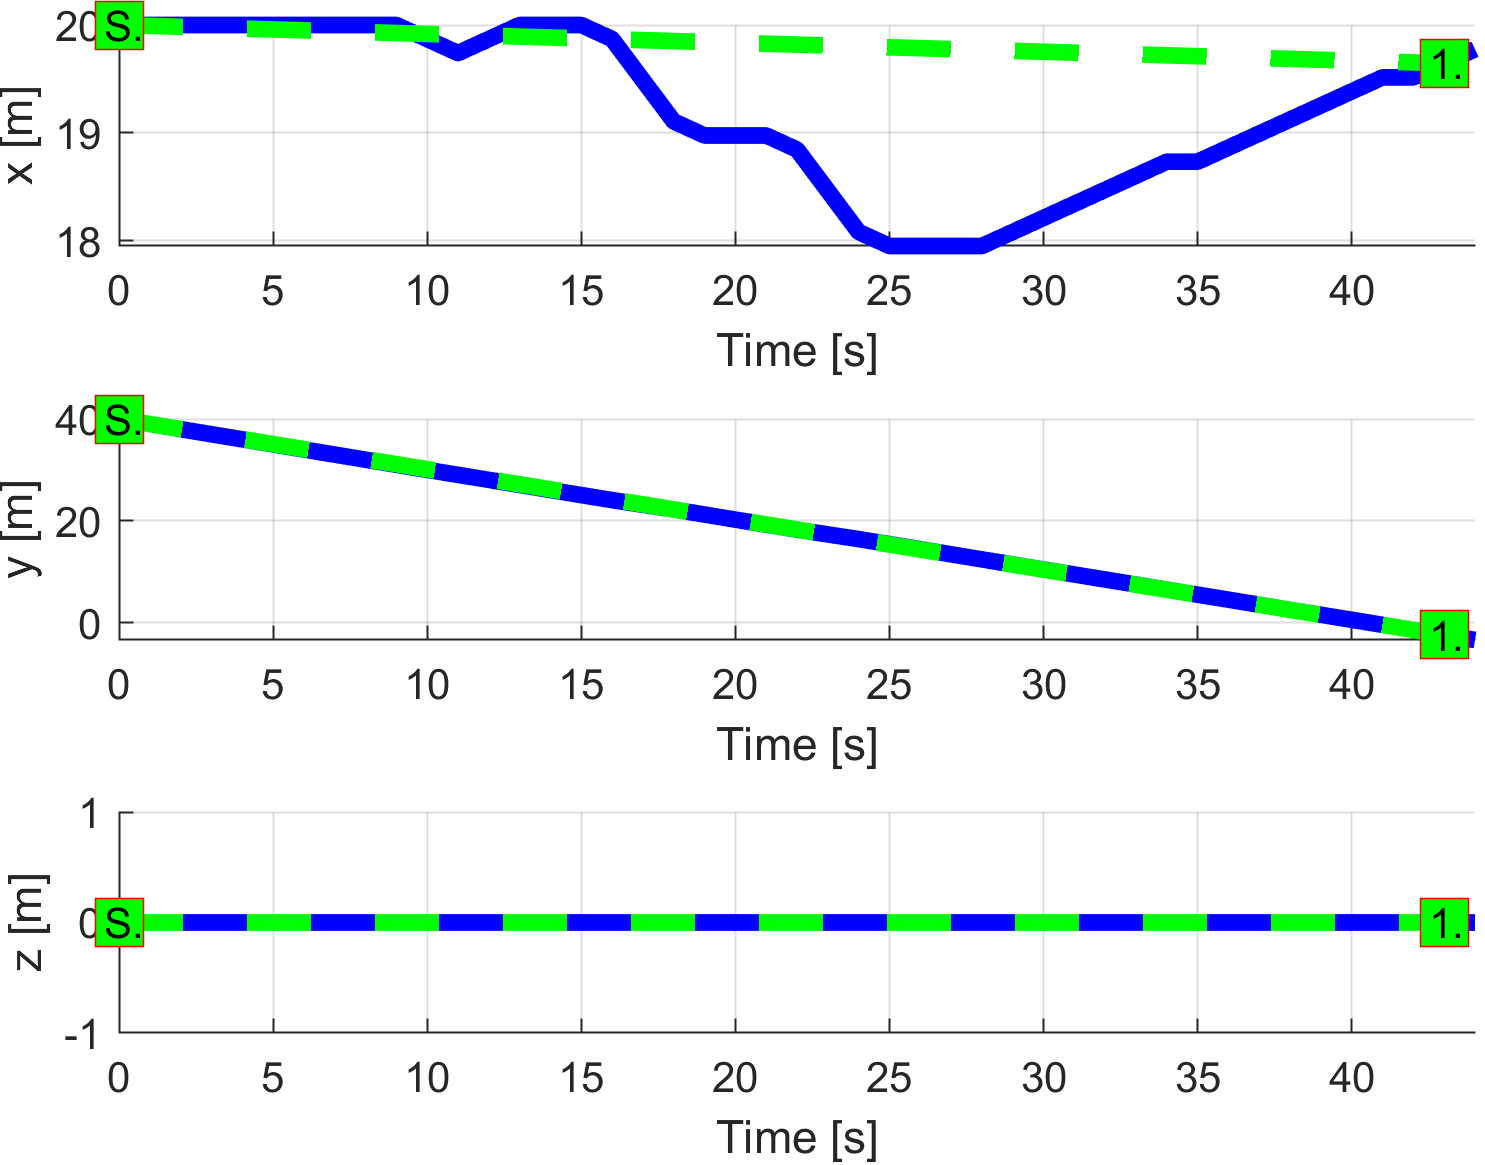
\includegraphics[width=0.9\linewidth]{\FIGDIR/NS047UtmEmergencyHeadOnMultipleUAV4PathFollowing} 
            \caption{UAS 4.}
            \label{fig:emergencyMixedPathTrackingUAS3}
        \end{subfigure}
        \caption{Trajectory tracking for \emph{Emergency mixed} situation test case.}
        \label{fig:testCaseEmergencyMixedTrajectoryTracking}
    \end{figure}
    
    \noindent\paragraph{Path Tracking Deviations:} \emph{Deviations} (tab. \ref{tab:pathTrackingParametersForEmergencyMixed}) are in expected ranges considering the \emph{mission plans} (tab. \ref{tab:missionSetupEmergencyMixedScenario}) and \emph{separation safety margins} (tab. \ref{tab:aboidanceParametersForEmergencyMixedScenario}).
    
    \begin{table}[H]
        \centering
        \begin{tabular}{c||c|c|c|c}
            \multirow{2}{*}{Param.} & UAS 1     & UAS 2             & UAS 3             & UAS 4 \\\cline{2-5}
                            & $\mathscr{WP}_1$  & $\mathscr{WP}_1$  & $\mathscr{WP}_1$  & $\mathscr{WP}_1$ \\\hline\hline
              $\max |x|$    & 0                 & 0                 & 1.98              & 2.05\\\hline
              $\max |y|$    & 4.84              & 0                 & 0                 & 0\\\hline
              $\max |z|$    & 0                 & 1.23              & 2.43              & 0\\\hline
              $\max dist.$  & 4.84              & 1.23              & 3.45              & 2.05\\
        \end{tabular}
        \caption{Path tracking properties for \emph{Emergency mixed} scenario.}
        \label{tab:pathTrackingParametersForEmergencyMixed}
    \end{table}    


% 07 Emergency Multiple
\paragraph{Computation Load:} The \emph{computation load} for \emph{scenario} (fig.\ref{fig:emergencyHeadOnMultipleComputationTime}) shows used time (y-axis) over decision frame (x-axis).

The \emph{computation time} increases during periods of \emph{active avoidance}. The \emph{shortest} period of avoidance has UAS 1 and the longest period of avoidance has UAS 4.

\begin{figure}[H]
    \centering
    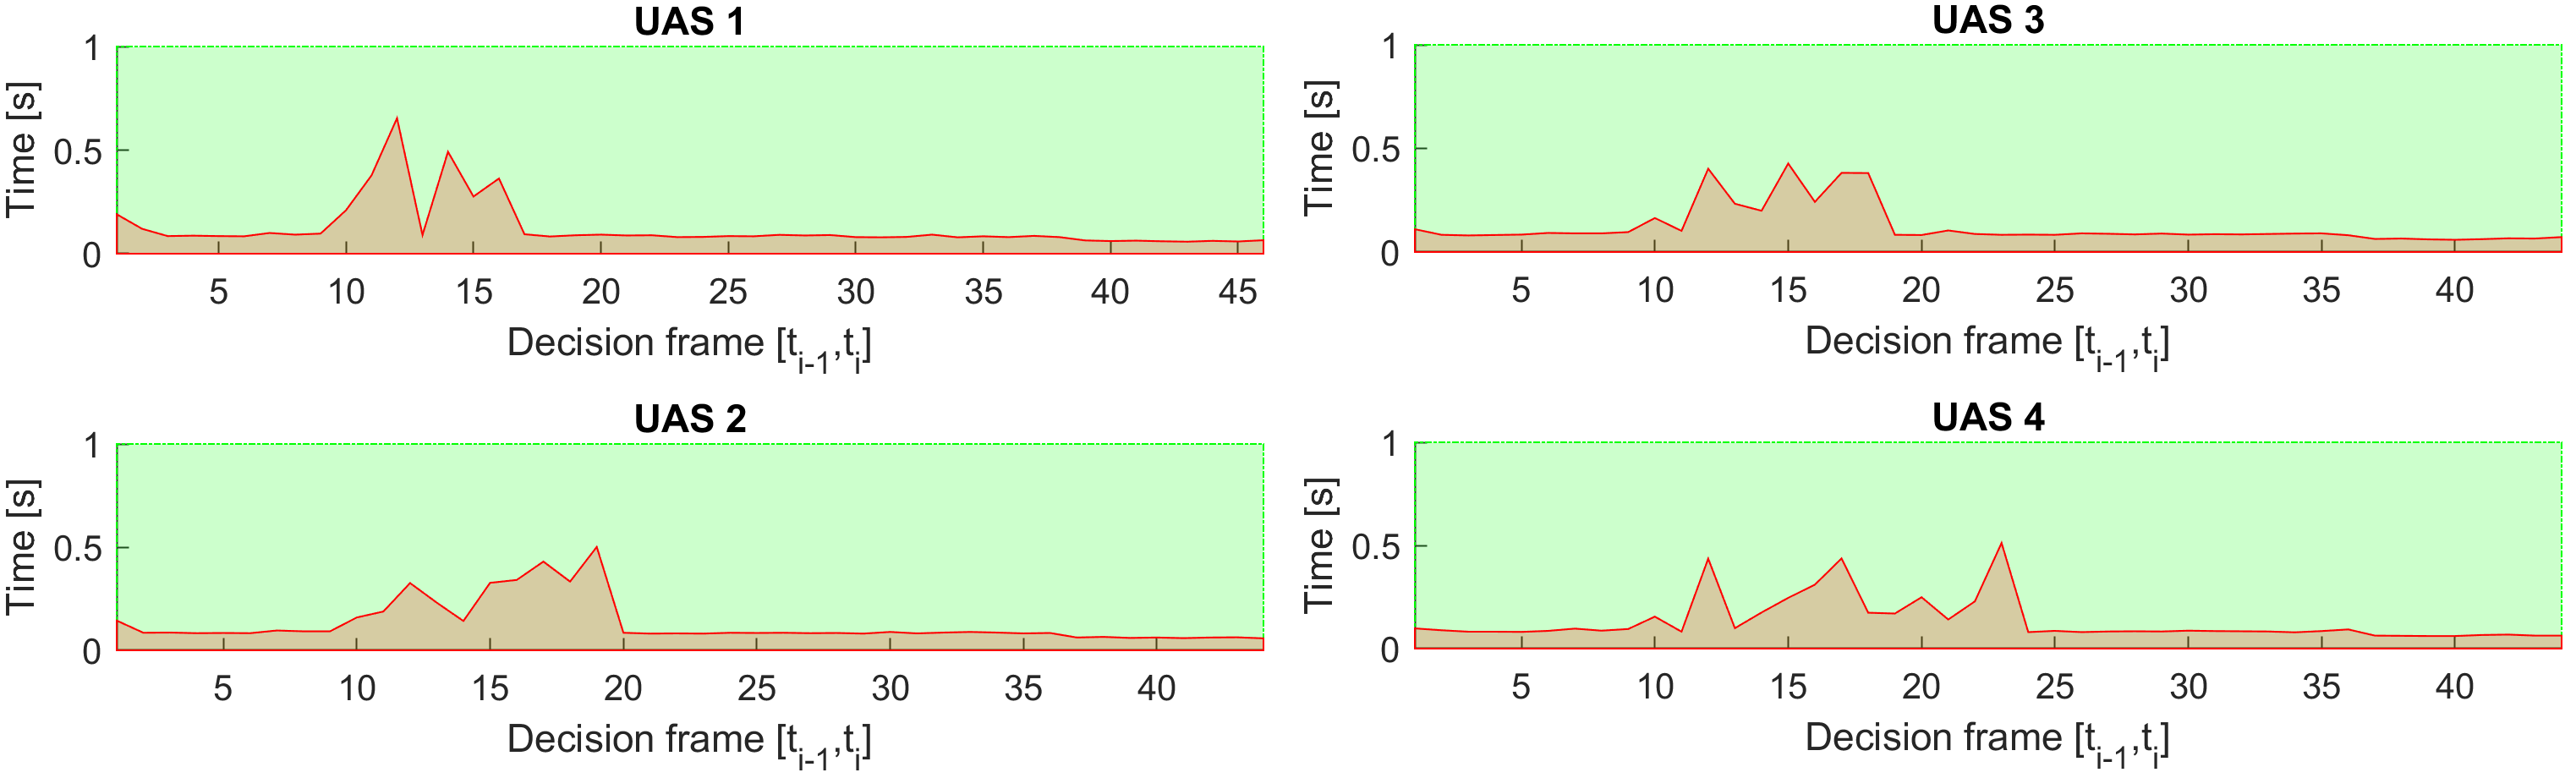
\includegraphics[width=0.95\linewidth]{\FIGDIR/NS098EmergencyHeadOnMultipleComputationTime} 
    \caption{Computation time for \emph{Emergency multiple} scenario.}
    \label{fig:emergencyHeadOnMultipleComputationTime}
\end{figure}

